\documentclass{report}

\usepackage{graphicx}
\usepackage{hyperref}

\graphicspath{{./assets/}}

\title{SER-210 Final: Design Report}
\author{Thomas Kwashnak}



\begin{document}
\maketitle

\tableofcontents
\newpage

\chapter{Introduction}

\section{About the App}
The app described in this report is an attempt at making an easy go-to chat app to communicate with team members when working on a Github account. It aims to provide quick and easy chat rooms for each repositoriy, while only requiring the user to have a Github account.

\section{Report Purpose}
The purpose of this report is to provide an outline of plans made for the creation of the app. This report contains the UI Design plans, System Design plans, as well as an overview on the production plan over 3 iterations.

\newpage
\section{User Stories}
\textit{Last Modified: 4/13/2022}
\begin{itemize}
    \item As a user, I can sign in with my GitHub account to sign into the app
    \item As a user, I can view a list of recent chat rooms to quickly get back to what I was working on
    \item As a user, I can tap a star on a chat room to pin it to the top of the list so I have easy access to chat rooms I want
    \item As a user, I can select a chat room to open it up
    \item As a user, I can type and send a message into the chat room to interact with the conversation
    \item As a user, I can see chat messages appear so I can keep up with the conversation
    \item As a user, I can share a chat so I can invite friends into the chat
    \item As a user, I can create a new chat room for a repository that I own so I can coordinate with other contributors
    \item As a user, I can type \# to reference a pull request or issue so viewers can click and navigate to that pull request or issue
    \item As a user, I can leave a chat room so I am not cluttered with chats I don't participate in
    \item As a user, I can view the app info so I know the app version and other information regarding the app
    \item As a user, I can log out of my account so I can log into another account
    \item As a user, I can click a link to redirect to the repository page from the chat info
\end{itemize}

\chapter{UI Design}

\section{Navigation Map}
\begin{center}
    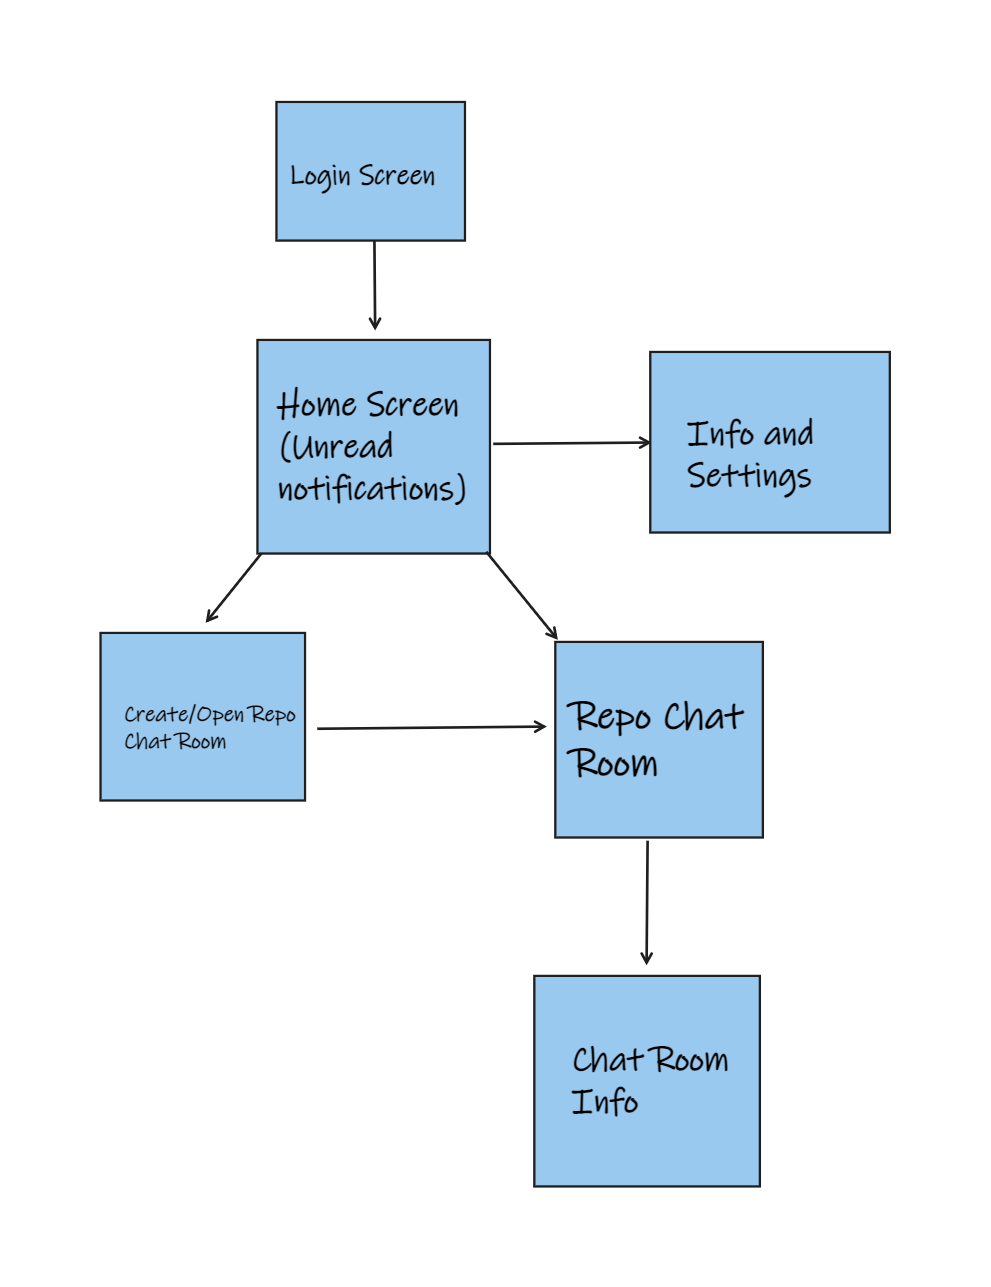
\includegraphics[width=\textwidth]{nav-graph}
\end{center}


\section{App Wireframes}

\subsection{Login Page}

\begin{center}
    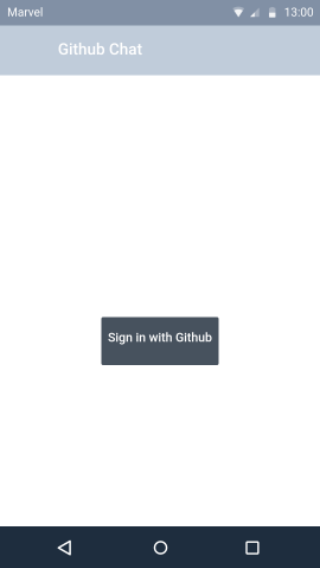
\includegraphics[scale=0.5]{design-login}
\end{center}
This is the landing page for the app after it first opens. If the user is signed in, then this page is bypassed. Otherwise, the user must sign in using their Github account.

\newpage
\subsection{Home Screen}

\begin{center}
    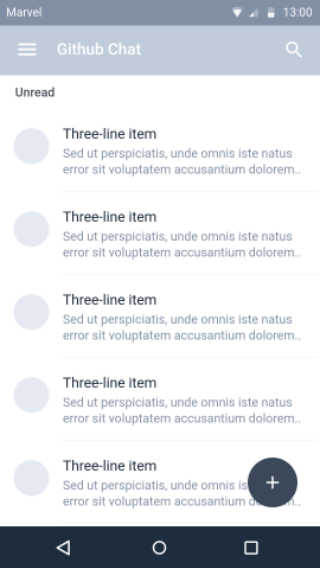
\includegraphics[scale=0.5]{design-home}
\end{center}

This is the home page. A list of recent repositories shows recent activity. A floating action button allows the user to create a new chat room for a repo. The user can select a "star" icon in order to "favorite" a chat

\newpage
\subsection{Navigation Drawer}

\begin{center}
    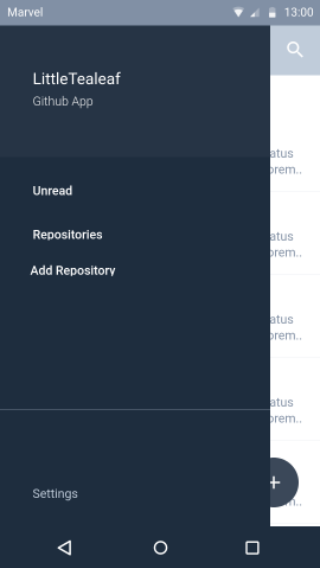
\includegraphics[scale=0.5]{design-nav-drawer}
\end{center}
The navigation drawer allows the user to access standard features such as adding repositories and opening settings


\newpage
\subsection{Options Screen}
\begin{center}
    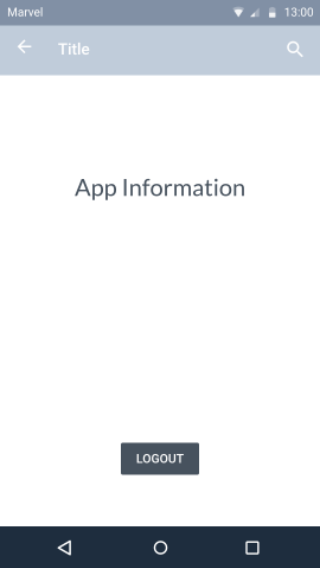
\includegraphics[scale=0.5]{design-options}
\end{center}
This screen displays the app information, and allows the user to log out of their account

\newpage
\subsection{Create Chat Screen}
\begin{center}
    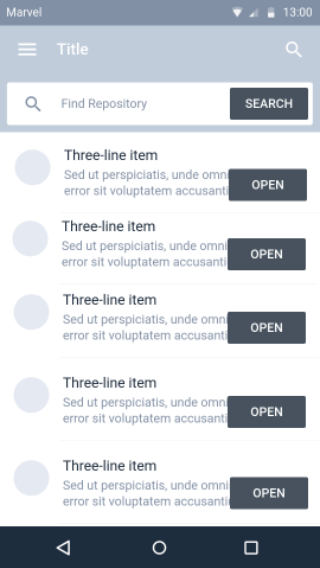
\includegraphics[scale=0.5]{design-create-chat}
\end{center}
This screen lists repositories the user owns, and the option to create a new chat room. The user can alternatively search up any repository to create a chat room for that repository.

\newpage
\subsection{Chat Screen}
\begin{center}
    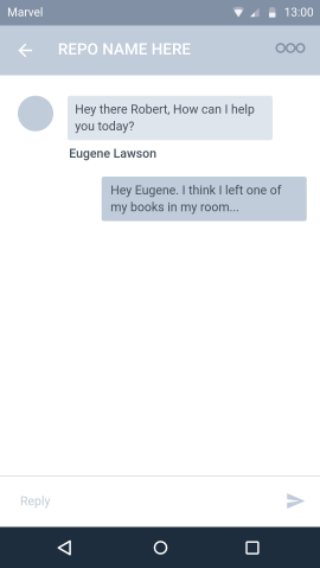
\includegraphics[scale=0.5]{design-chat}
\end{center}

This screen shows the actual chat room. The user can type a message into the message box. By typing \#, the user can link an issue or pull request.

\newpage
\subsection{Chat Info Screen}
\begin{center}
    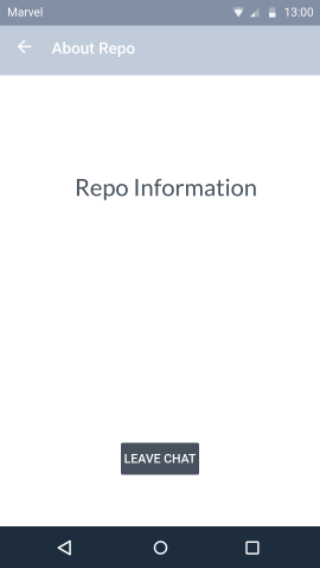
\includegraphics[scale=0.5]{design-chat-info}
\end{center}
This screen shows common repository information, as well as a link the user can use to navigate to the repository. Additionally, the user can click the leave chat to remove the chat from their list.

\newpage
\section{User Story Coverage}

\begin{center}
    \begin{tabular}{ | p{0.9\linewidth} |}
        \hline
        \textbf{Login Screen} \begin{itemize}
                                  \item As a user, I can sign in with my GitHub account to sign into the app
                              \end{itemize}                                                        \\
        \hline
        \textbf{Home Screen} \begin{itemize}
                                 \item As a user, I can view a list of recent chat rooms to quickly get back to what I was working on
                                 \item As a user, I can tap a star on a chat room to pin it ot the top of the list so I can keep chat rooms I want to keep on top
                                 \item As a user, I can select a chat room to open it up
                             \end{itemize}   \\
        \hline
        \textbf{Create Chat Screen}\begin{itemize}
                                       \item As a user, I can create a new chat room for a repository that I own so I can coordinate with other contributors
                                   \end{itemize}        \\
        \hline
        \textbf{Chat Screen}\begin{itemize}
                                \item As a user, I can type and send a message into the chat room to interact with the conversation
                                \item As a user, I can see chat messages appear so I can keep up with the conversation
                                \item As a user, I can type \# to reference a pull request or issue so viewers can click and navigate to that pull request or issue

                            \end{itemize} \\
        \hline
        \textbf{Chat Info Screen}\begin{itemize}
                                     \item As a user, I can share a chat room so my friends can join
                                     \item As a user, I can click a link to redirect to the repository page from the chat info
                                 \end{itemize}                                      \\
        \hline
        \textbf{Options Screen}\begin{itemize}
                                   \item As a user, I can log out of my account so I can log into another account
                                   \item As a user, I can view the app info so I know the app version and other information regarding the app

                               \end{itemize}                       \\
        \hline
    \end{tabular}
\end{center}

\chapter{System Design}

\section{Database Design}

\subsubsection{Messages}
\begin{tabular}{| l | l | l |}
    \hline
    \textbf{Name} & \textbf{Type} & \textbf{Key} \\
    \hline
    \hline
    \_id          & Integer       & Primary Key  \\
    \hline
    message       & String        & Not Null     \\
    \hline
    time          & Integer       & Not Null     \\
    \hline
    sender        & String        & Not Null     \\
    \hline
    apiSender     & Integer       & Foreign Key  \\
    \hline
    repository    & Integer       & Foreign Key  \\
    \hline
    isRead        & Boolean       &              \\
    \hline
\end{tabular}
\subsubsection{Repositories (Chat Rooms)}
\begin{tabular}{| l | l | l |}
    \hline
    \textbf{Name} & \textbf{Type} & \textbf{Key} \\
    \hline
    \hline
    \_id          & Integer       & Primary Key  \\
    \hline
    name          & String        & Not Null     \\
    \hline
    apiRepo       & Integer       & Foreign Key  \\
    \hline
    apiPulls      & Integer       & Foreign Key  \\
    \hline
    apiIssues     & Integer       & Foreign Key  \\
    \hline
    isFavorite    & Boolean       &              \\
    \hline
\end{tabular}

\subsubsection{Github API Cache}
\begin{tabular}{| l | l | l |}
    \hline
    \textbf{Name} & \textbf{Type} & \textbf{Key} \\
    \hline
    \hline
    \_id          & Integer       & Primary Key  \\
    \hline
    url           & String        & Not Null     \\
    \hline
    content       & String        & Not Null     \\
    \hline
    fetchTime     & Integer       & Not Null     \\
    \hline
\end{tabular}

\section{Class Diagram}

\begin{center}
    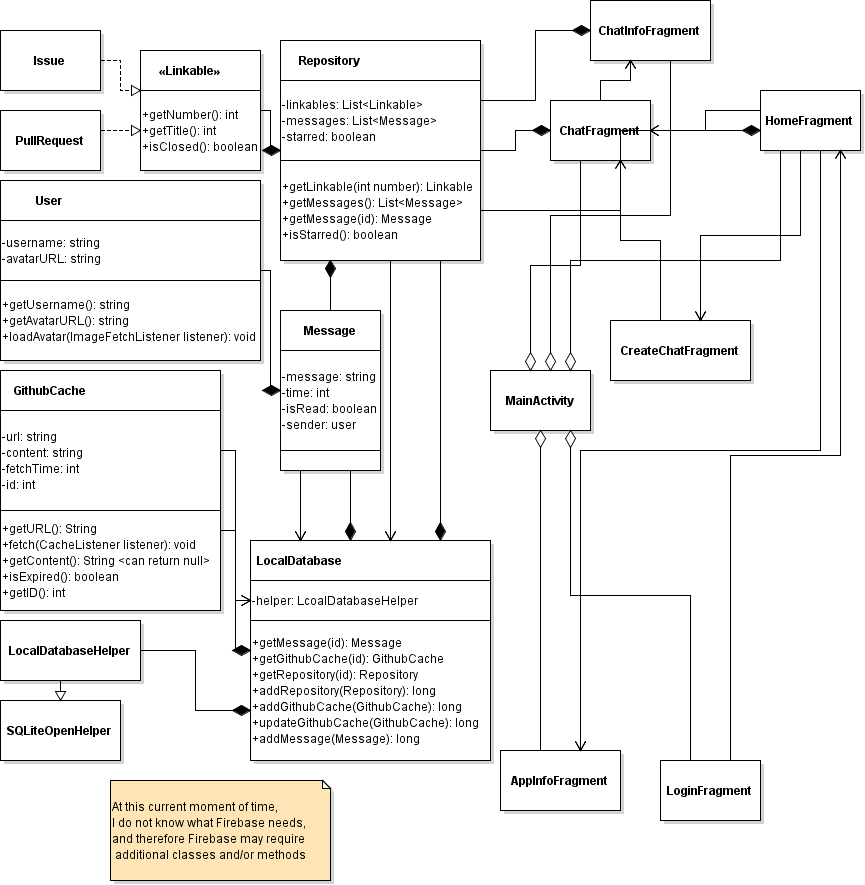
\includegraphics[scale=0.4]{uml-diagram}
\end{center}
You can view the full diagram at \href{https://github.com/LittleTealeaf/SER-210-Final/blob/main/docs/reports/design/assets/uml-diagram.png}{https://github.com/LittleTealeaf/SER-210-Final/blob/main/docs/reports/design/assets/uml-diagram.png}\\

The class diagram is my current understanding of how the classes will be set up. In terms of the back-end, the Repository, GithubCache, and Message repositories are all generated directly from the LocalDatabase (I'll probably come up with a better name by then). The local database supports adding and retrieving Repositories, Messages, and Github Caches. The local database also supports updating GithubCaches with fresh values, which uses an interface to support the async task.

\section{Class User Stories}

\begin{center}
    \begin{tabular}{ | p{0.9\linewidth} |}
        \hline
        \textbf{LoginFragment} \begin{itemize}
                                   \item As a user, I can sign in with my GitHub account to sign into the app
                               \end{itemize}                                                       \\
        \hline
        \textbf{ChatFragment} \begin{itemize}
                                  \item I can view a list of recent chat rooms to quickly get back to what I was working on
                                  \item As a user, I can type and send a message into the chat room to interact with the conversation
                                  \item As a user, I can see chat messages appear so I can keep up with the conversation
                                  \item I can tap a star on a chat room to pin it to the top of the list so I have easy access to chat rooms I want
                                  \item As a user, I can share a chat so I can invite friends into the chat
                              \end{itemize}                 \\
        \hline
        \textbf{ChatInfoFragment} \begin{itemize}
                                      \item As a user, I can click a link to redirect to the repository page from the chat info
                                      \item As a user, I can leave a chat room so I am not cluttered with chats I don't participate in
                                  \end{itemize}                                     \\
        \hline
        \textbf{AppInfoFragment} \begin{itemize}
                                     \item As a user, I can view the app info so I know the app version and other information regarding the app
                                 \end{itemize}                     \\
        \hline
        \textbf{Repository} \begin{itemize}
                                \item As a user, I can type \# to reference a pull request or issue so viewers can click and navigate to that pull request or issue
                            \end{itemize} \\
        \hline
        \textbf{CreateChatFragment} \begin{itemize}
                                        \item As a user, I can create a new chat room for a repository that I own so I can coordinate with other contributors
                                    \end{itemize}       \\
        \hline
        \textbf{HomeFragment} \begin{itemize}
                                  \item As a user, I can view a list of recent chat rooms to quickly get back to what I was working on
                                  \item As a user, I can select a chat room to open it up
                              \end{itemize}                              \\
        \hline
        \textbf{AppInfoFragment} \begin{itemize}
                \item As a user, I can log out of my account so I can log into another account
        \end{itemize} \\
        \hline
    \end{tabular}
\end{center}



\chapter{Iteration Planning}

\section{Prioritized User Stories}

User stories below are sorted from most to least prioritized

\begin{enumerate}
    \item As a user, I can sign in with my GitHub account to sign into the app
    \item As a user, I can type and send a message into the chat room to interact with the conversation
    \item As a user, I can see chat messages appear so I can keep up with the conversation
    \item As a user, I can create a new chat room for a repository that I own so I can coordinate with other contributors
    \item As a user, I can view a list of recent chat rooms to quickly get back to what I was working on
    \item As a user, I can select a chat room to open it up
    \item As a user, I can type \# to reference a pull request or issue so viewers can click and navigate to that pull request or issue
    \item As a user, I can leave a chat room so I am not cluttered with chats I don't participate in
    \item As a user, I can tap a star on a chat room to pin it to the top of the list so I have easy access to chat rooms I want
    \item As a user, I can view the app info so I know the app version and other information regarding the app
    \item As a user, I can click a link to redirect to the repository page from the chat info
    \item As a user, I can log out of my account so I can log into another account
    \item As a user, I can share a chat so I can invite friends into the chat
\end{enumerate}


\end{document}
